\documentclass[12pt]{scrreprt} 
\usepackage{graphicx}
\usepackage{tikz}
\usepackage{mathtools}
\usepackage{caption}
\captionsetup[figure]{labelformat=empty}
\usetikzlibrary{automata,positioning}
\PassOptionsToPackage{usenames,dvipsnames,svgnames}{xcolor}


\begin{document} 

\begin{titlepage}

\newcommand{\HRule}{\rule{\linewidth}{0.5mm}} % Defines a new command for the horizontal lines, change thickness here

\center % Center everything on the page

%----------------------------------------------------------------------------------------
%	HEADING SECTIONS
%----------------------------------------------------------------------------------------

\textsc{\LARGE University of North Alabama}\\[1.5cm] % Name of your university/college
\textsc{\Large Programming Languages}\\[0.5cm] % Major heading such as course name

%----------------------------------------------------------------------------------------
%	TITLE SECTION
%----------------------------------------------------------------------------------------

\HRule \\[0.4cm]
{ \huge \bfseries JavaScript}\\[0.4cm] % Title of your document
\HRule \\[1.5cm]
 
%----------------------------------------------------------------------------------------
%	AUTHOR SECTION
%----------------------------------------------------------------------------------------

\begin{minipage}{0.4\textwidth}
\begin{flushleft} \large
\emph{Author:}\\
Jeffrey \textsc{Allen}
\end{flushleft}
\end{minipage}
~
\begin{minipage}{0.4\textwidth}
\begin{flushright} \large
\emph{Professor:} \\
Dr. Patricia \textsc{Roden}
\end{flushright}
\end{minipage}\\[4cm]

{\large \today}\\[3cm] % Date, change the \today to a set date if you want to be precise

\vfill % Fill the rest of the page with whitespace

\end{titlepage}

\tableofcontents 

\chapter{Graph Theory and Matrices} 

\begin{figure}[h]
	
	\centering
		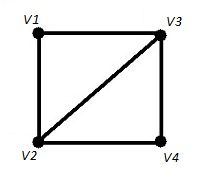
\includegraphics[width=0.25\textwidth]{figure1}
	\caption{Figure 1}

\end{figure}

\section{Adjacency matrix for $A$} 

\[ A = \left( \begin{array}{cccc}
0 & 1 & 1 & 0 \\
1 & 0 & 1 & 1 \\
1 & 1 & 0 & 1 \\
0 & 1 & 1 & 0 \end{array} \right)\] 

\section{$A^2$ and $A^3$}

\[ A^2 = \left( \begin{array}{cccc}
2 & 1 & 1 & 2 \\
1 & 3 & 2 & 1 \\
1 & 2 & 3 & 1 \\
2 & 1 & 1 & 2 \end{array} \right)\] 

\[ A^3 = \left( \begin{array}{cccc}
2 & 5 & 5 & 2 \\
5 & 4 & 5 & 5 \\
5 & 5 & 4 & 5 \\
2 & 5 & 5 & 2 \end{array} \right)\] 

\pagebreak

\subsection{What values in $A^n$ tell about the graph in Figure 1 & proving your claim for $A^2$} 

The $n$ in the expression $A^n$ represents the amount of edges that must be used in order to travel between one  node, to another.
The adjacency matrix for $A^1$ represents $0$ paths between $V_1$ and itself. In the adjacency matrix $A^2$, there are
$2$ possible paths from $V_1$ to itself utilizing 2 edges.

\section{Compute the eigenvalues and eigenvectors for $A$}

  \begin{center}
  \textbf{Eigenvalues}
  \end{center}

  \begin{center}
  \begin{tabular}{ c c c p{5cm} }
    $\lambda_1$ & $\rightarrow$ & $\frac{1}{2}(1+\sqrt{17})$ \\        
    $\lambda_2$ & $\rightarrow$ & $\frac{1}{2}(1-\sqrt{17})$ \\
    $\lambda_3$ & $\rightarrow$ & -1 \\
    $\lambda_4$ & $\rightarrow$ & 0 \\
  \end{tabular}
  \end{center}

  \begin{center}
  \textbf{Eigenvectors}
  \end{center}

  \begin{center}
  $\vec{x}_1 = \begin{pmatrix}1\\\frac{1}{4}(1 + \sqrt{17})\\\frac{1}{4}(1 + \sqrt{17})\\1\end{pmatrix}$
  $\vec{x}_2 = \begin{pmatrix}1\\\frac{1}{4}(1 - \sqrt{17})\\\frac{1}{4}(1 - \sqrt{17})\\1\end{pmatrix}$
  $\vec{x}_3 = \begin{pmatrix}0\\-1\\1\\0\end{pmatrix}$
  $\vec{x}_4 = \begin{pmatrix}-1\\0\\0\\1\end{pmatrix}$
  \end{center}

\subsection{Importance of eigenvalues and eigenvectors to graph}

We observed that there is one zero, one positive, and two negative eigenvalues for the adjacency matrix $A$.
The importance of these values related to the graph can be used to determine the structure of the graph.
For this graph, 

\pagebreak

\begin{figure}[h]
	\centering
		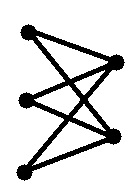
\includegraphics[width=0.25\textwidth]{figure2}
	\caption{Figure 2}
\end{figure}

\section{Draw the adjacency matrix $A$ for Figure 2}

\[ \left( \begin{array}{ccccc}
0 & 1 & 0 & 1 & 0 \\
1 & 0 & 1 & 0 & 1 \\
0 & 1 & 0 & 1 & 0 \\
1 & 0 & 1 & 0 & 1 \\
0 & 1 & 0 & 1 & 0 \end{array} \right)\] 

\section{Figure 2 Cycles} 
\subsection{Amount of 2-cycles for the left-hand and right-hand vertices}

\centerline{Left-hand: 6}
\centerline{Right-Hand: 6}

\subsection{Amount of 4-cycles for the left-hand and right-hand vertices} 

\centerline{Left-hand: 6}
\centerline{Right-Hand: 4}

\subsection{Amount of 6-cycles for the left-hand and right-hand vertices} 

\centerline{Left-hand: 0}
\centerline{Right-Hand: 0}

\pagebreak

\section{Eigenvalues and eigenvectors for graph in Figure 2}

  \begin{center}
  \textbf{Eigenvalues}
  \end{center}

  \begin{center}
  \begin{tabular}{ c c c p{5cm} }
    $\lambda_1$ & $\rightarrow$ & $-\sqrt{6}$ \\        
    $\lambda_2$ & $\rightarrow$ & $\sqrt{6}$ \\
    $\lambda_3$ & $\rightarrow$ & 0 \\
    $\lambda_4$ & $\rightarrow$ & 0 \\
    $\lambda_3$ & $\rightarrow$ & 0 \\
  \end{tabular}
  \end{center}

  \begin{center}
  \textbf{Eigenvectors}
  \end{center}

  \begin{center}
  $\vec{x}_1 = \begin{pmatrix}\\1\\\sqrt{\frac{3}{2}}\\1\\\sqrt{\frac{3}{2}}\\1\end{pmatrix}$
  $\vec{x}_1 = \begin{pmatrix}\\1\\-\sqrt{\frac{3}{2}}\\1\\-\sqrt{\frac{3}{2}}\\1\end{pmatrix}$
  $\vec{x}_3 = \begin{pmatrix}-1\\0\\0\\0\\1\end{pmatrix}$
  $\vec{x}_4 = \begin{pmatrix}0\\-1\\0\\1\\0\end{pmatrix}$
  $\vec{x}_5 = \begin{pmatrix}-1\\0\\1\\0\\0\end{pmatrix}$
  \end{center}
\subsection{Importance of eigenvalues and eigenvectors}

The eigenvalues and eigenvectors explain the structure of the graph. Observing
that the greatest eigenvalue is positive form of the smallest eigenvalue for this graph,
we can conclude that this graph is Bi-partite.

\section{$k$-paths from A to B when $k=1,2,3,4,5,6$}

\begin{center}
$k = 1 \rightarrow$ 0 \\
$k = 2 \rightarrow$ 1 \\
$k = 3 \rightarrow$ 0 \\
$k = 4 \rightarrow$ 4 \\
$k = 5 \rightarrow$ 0 \\
$k = 6 \rightarrow$ 6 \\
\end{center}

\section{Properties Figure 3 has in common with Figure 2}

These two graphs share the property of their respective adjacency matrices being
symmetric.

\pagebreak

\section{Eigenvalues of the $n$-cube for $n=1,2,3,4$}

	\begin{center}
		$n = 1$
	\end{center}

	\vspace{.1 mm}

	\begin{center}
	\begin{tabular}{ c c c p{5cm} }
    $\lambda_1$ & $\rightarrow$ & $1$ \\
	\end{tabular}
	\end{center}

	\begin{center}
		\line(1,0){250}\\
		$n = 2$
	\end{center}

	\vspace{.1 mm}

  \begin{center}
  \begin{tabular}{ c c c p{5cm} }
    $\lambda_1$ & $\rightarrow$ & -2 \\        
    $\lambda_2$ & $\rightarrow$ & 2 \\
    $\lambda_3$ & $\rightarrow$ & 0 \\
    $\lambda_4$ & $\rightarrow$ & 0 \\
  \end{tabular}
  \end{center}

	\vspace{.1 mm}

	\begin{center}
		\line(1,0){250}\\
		$n = 3$
	\end{center}

	\vspace{.1 mm}

	\begin{center}
	\begin{tabular}{ c c c p{5cm} }
	$\lambda_1$ & $\rightarrow$ & -3 \\
	$\lambda_2$ & $\rightarrow$ &  3 \\
	$\lambda_3$ & $\rightarrow$ & -1 \\
	$\lambda_4$ & $\rightarrow$ & -1 \\
	$\lambda_5$ & $\rightarrow$ &  1 \\
	$\lambda_6$ & $\rightarrow$ &  1 \\
	$\lambda_7$ & $\rightarrow$ &  0 \\
	$\lambda_8$ & $\rightarrow$ &  0 \\
	\end{tabular}
	\end{center}

	\begin{center}
		$n = 4$
	\end{center}

	\vspace{.1 mm}

	\begin{center}
	\begin{tabular}{ c c c p{5cm} }
	$\lambda_1$ & $\rightarrow$ &  0 \\
	$\lambda_2$ & $\rightarrow$ &  0 \\
	$\lambda_3$ & $\rightarrow$ &  0 \\
	$\lambda_4$ & $\rightarrow$ &  0 \\
	$\lambda_5$ & $\rightarrow$ &  0 \\
	$\lambda_6$ & $\rightarrow$ &  0 \\
	$\lambda_7$ & $\rightarrow$ & -2 \\
	$\lambda_8$ & $\rightarrow$ & -2 \\
	$\lambda_1$ & $\rightarrow$ & -2 \\
	$\lambda_2$ & $\rightarrow$ & -2 \\
	$\lambda_3$ & $\rightarrow$ &  2 \\
	$\lambda_4$ & $\rightarrow$ &  2 \\
	$\lambda_5$ & $\rightarrow$ &  2 \\
	$\lambda_6$ & $\rightarrow$ &  2 \\
	$\lambda_7$ & $\rightarrow$ & -4 \\
	$\lambda_8$ & $\rightarrow$ &  4 \\
	\end{tabular}
	\end{center}


\chapter{Digraphs and Ranking} 

\begin{figure}[h]
	\centering
		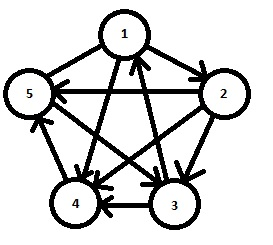
\includegraphics[width=0.25\textwidth]{figure4}
	\caption{Figure 4}
\end{figure}


\section{Draw the Transition Matrix $A$ for Figure 4}

\[ A = \left( \begin{array}{ccccc}
0 & 1 & 0 & 1 & 1 \\
0 & 0 & 1 & 1 & 1 \\
1 & 0 & 0 & 1 & 0 \\
0 & 0 & 0 & 0 & 1 \\
0 & 0 & 1 & 0 & 0 \end{array} \right)\] 

\section{Compute $A^2$ and $A^3$}

\[ A^2 = \left( \begin{array}{ccccc}
0 & 0 & 2 & 1 & 2 \\
1 & 0 & 1 & 1 & 1 \\
0 & 1 & 0 & 1 & 2 \\
0 & 0 & 1 & 0 & 0 \\
1 & 0 & 0 & 1 & 0 \end{array} \right)\] 

\[ A^3 = \left( \begin{array}{ccccc}
2 & 0 & 2 & 2 & 1 \\
1 & 1 & 1 & 2 & 2 \\
0 & 0 & 3 & 1 & 2 \\
1 & 0 & 0 & 1 & 0 \\
0 & 2 & 0 & 1 & 2 \end{array} \right)\] 


\subsection{What are the values in $A^n$ telling you about the graph in Figure 1? Prove your claim for $A^2$}

The $n$ in $A^n$ represents the number of edges that must be used in order to travel from one vertice to another.
Referring to Figure 2, it is apparent that there doesn't exist a path $V1 \rightarrow V3$. However, the adjacency matrix $A^2$
calculates that there are 2 paths $V1 \rightarrow V3$. This is because the adjacency matrix has defined paths between vertices
by utilizing 2 edges, such as $V1 \rightarrow V5 \rightarrow V3$ and $V1 \rightarrow V2 \rightarrow V3$.

\section{Round Robin Tournament using method described in class}

To illustrate the ideas introduced throughout this section, the digraph in Figure 2 will be viewed as a Street Fighter tournament where each
vertice will be imagined as a player. The edge stemming from one vertice to another will represent a match played between players
that will result in a win for one player, and a loss for the other. The player that wins will have its edge directed at the losing player.
Taking the graph in Figure 2 and applying Person-Frobineus theorem to the tournament matrix, it can be calculated that the ranks of the players are:

\begin{center}
	1st: Player 1 \\
	2nd: Player 2 \\
	3rd: Player 3 \\
	4th: Player 5 \\
	5th: Player 4 \\
\end{center}

\subsection{Method}

Since we are interested in the rankings of the players, we first organize the rankings of the players into a $ranking vector \vec{r}$.

\[ r = \begin{pmatrix}r_1\\r_2\\r_3\\r_4\\r_5\end{pmatrix} \]

Then, we associate the amount of wins with a player by setting $\vec{r} = A$. This yielded the
following system

\[ r_1 = \alpha(r_2 + r_4 + r_5) \]
\[ r_2 = \alpha(r_3 + r_4 + r_5)\]
\[ r_3 = \alpha(r_1 + r_4)\]
\[ r_4 = \alpha(r_1)\]
\[ r_5 = \alpha(r_3)\]

By manipulating this system, we transformed the equation

\[\vec{r} = \alpha A \vec{r}\]

to

 \[A\vec{r} = \frac{1}{\alpha}\vec{r} \]

 When the system is represented in this manner, along with the fact that $A$ turns
 out to be a nonnegative matrix, then it is possible to apply the Perron-Frobenius Theorem
 to find a solution to this ranking problem. The Perron-Frobenius Theorem guarantees that there is a $unique$
 ranking vector $\vec{r}$. Using this fact, we solved for corresponding eigenvalues and eigenvectors for the tournament
 matrix $A$. This produced the equation: 
 
 \[A\begin{pmatrix}2.15062\\1.96587\\1.6593\\0.602663\\1\end{pmatrix} = 1.6593\begin{pmatrix}2.15062\\1.96587\\1.6593\\0.602663\\1\end{pmatrix} \]

Multiplying the left hand side of each equation by $A^{-1}$, we see that we have solved
for the ranking vector $\vec{r}$

\[\begin{pmatrix}2.1\\1.9\\1.6\\0.6\\1\end{pmatrix} \rightarrow \vec{r_i} = \begin{pmatrix}1st\\2nd\\3rd\\5th\\4th\end{pmatrix} \]

\chapter{Automata and Matrices}

\section{Finite automata that accepts all strings that end with $ab$}

\begin{center}
	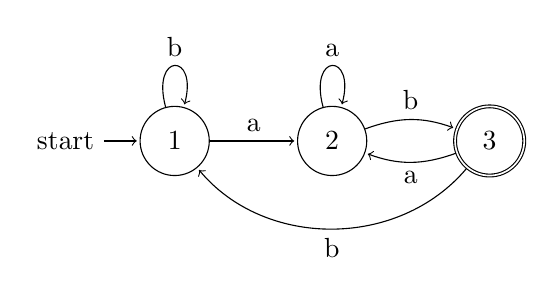
\begin{tikzpicture}[shorten >=1pt,node distance=2cm,on grid,auto] 
	   \node[state,initial] (q_0)   {$1$};
	   \node[state] (q_1) [right=of q_0] {$2$}; 
	   \node[state,accepting](q_2) [right=of q_1] {$3$}; 
	    \path[->] 
	    (q_0) edge  node {a} (q_1)
	    	  edge [loop above] node {b} ()
	    (q_1) edge [bend left=20] node  {b} (q_2)
	          edge [loop above] node {a} ()
	    (q_2) edge [bend left=20] node {a} (q_1)
	          edge [bend left=50] node {b} (q_0);
	\end{tikzpicture} 
\end{center}

\section{Finite automata that accepts all strings such that the number of $a's$ is divisible by 5, and the number of $b's$ is divisible by 3}

\begin{figure}[h]
	\centering
		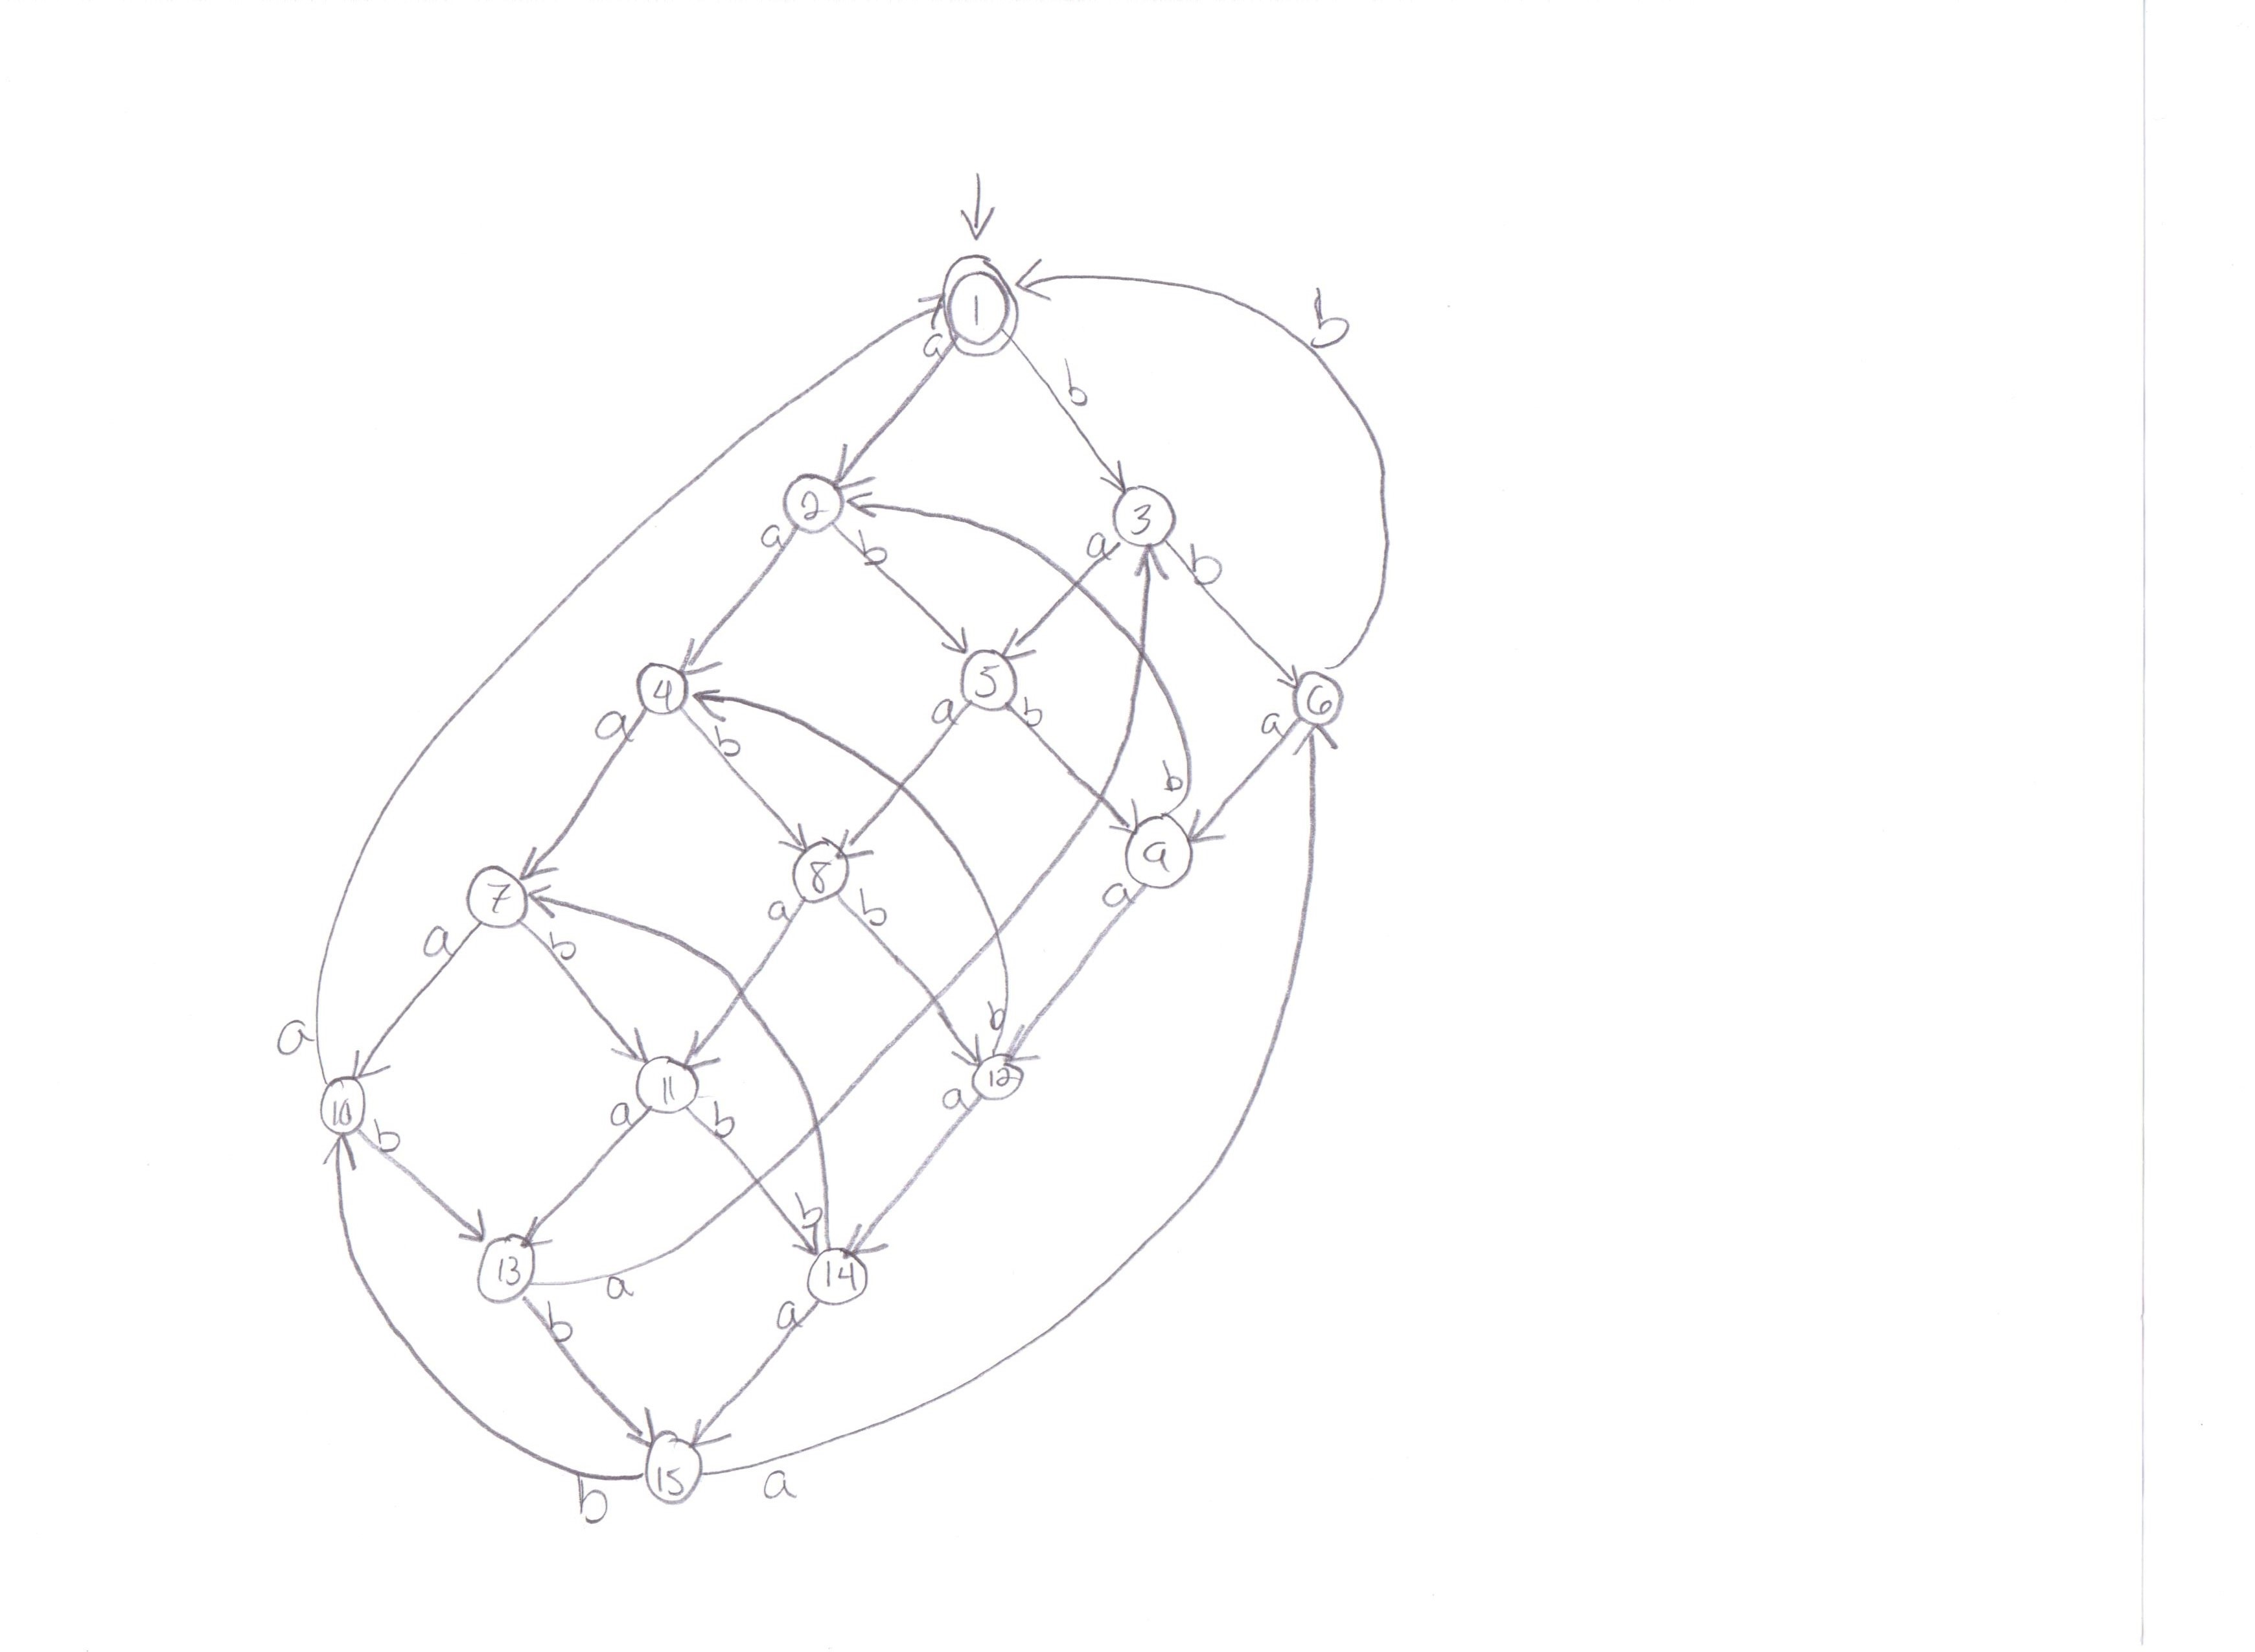
\includegraphics[width=0.78\textwidth]{3_2}
\end{figure}

\section{Finite automata that accepts all strings such that every block of 5 symbols contains at least two $a's$}

\begin{center}
	\begin{tikzpicture}[shorten >=1pt,node distance=3cm,on grid,auto] 
	   \node[state,initial,accepting] (q_0)   {$1$};
	   \node[state] (q_1) [right=of q_0] {$2$}; 
	   \node[state] (q_2) [right=of q_1] {$3$};
	   \node[state] (q_3) [below=of q_0] {$4$}; 
	   \node[state] (q_4) [right=of q_3] {$5$};
	   \node[state] (q_5) [right=of q_4] {$6$}; 
	   \node[state] (q_6) [right=of q_2] {$7$}; 
	   \node[state] (q_7) [below=of q_3] {$8$}; 
	   \node[state] (q_8) [right=of q_7] {$9$}; 
	   \node[state] (q_9) [below=of q_7] {$10$}; 
	   \node[state] (q_10) [right=of q_9] {$11$}; 
	   \node[state] (q_11) [below=of q_9] {$12$}; 
	    \path[->] 
	    (q_0) edge  node {a} (q_1)
	    	  edge  node {b} (q_3)
	    (q_1) edge  node {a} (q_2)
	          edge  node {b} (q_4)
	    (q_2) edge  node {a,b} (q_5)
	    (q_3) edge  node {a} (q_4)
	    	  edge  node {b} (q_7)
	    (q_4) edge  node {a} (q_5)
	    	  edge  node {b} (q_8)
	    (q_5) edge [bend right=45] node {a,b} (q_6)
	    (q_6) edge [bend right=40] node {a,b} (q_0)
	    (q_7) edge  node {a} (q_8)
	          edge  node {b} (q_9)
	    (q_8) edge  node {b} (q_10)
	          edge [bend right=60] node {a} (q_6)
	    (q_9) edge  node {a} (q_10)
	    	  edge  node {b} (q_11)
	    (q_10) edge node {a} (q_0)
	    	   edge node {b} (q_11)
	    (q_11) edge [loop below] node {a,b} ();
	\end{tikzpicture} 
\end{center}

\section{Strings that are accepted by automata in Figure 5}

\begin{figure}
\begin{center}
	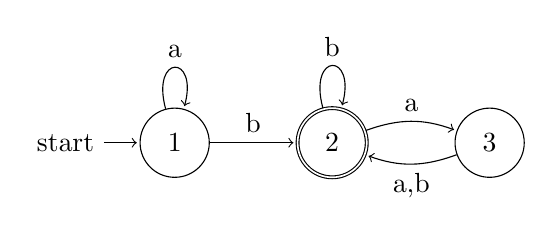
\begin{tikzpicture}[shorten >=1pt,node distance=2cm,on grid,auto] 
	   \node[state,initial] (q_0)   {$1$};
	   \node[state,accepting] (q_1) [right=of q_0] {$2$}; 
	   \node[state] (q_2) [right=of q_1] {$3$}; 
	    \path[->] 
	    (q_0) edge [loop above] node {a} ()
	    	  edge node {b} (q_1)
	    (q_1) edge [bend left=20] node  {a} (q_2)
	          edge [loop above] node {b} ()
	    (q_2) edge [bend left=20] node {a,b} (q_1);
	\end{tikzpicture} 
	\caption{Figure 5}
\end{center}
\end{figure}


The automata in Figure 5 accepts strings that must include atleast one $b$ and does not end with $ba$.
For all strings that do not include $b$, it is not possible to exit state 1.
All strings that end with $ba$ will finish at state 3.

\section{Transition matrix for automata in figure 5 labeled $A,B$}

\[ A = \left( \begin{array}{ccc}
1 & 0 & 0 \\
0 & 0 & 1 \\
0 & 1 & 0 \end{array} \right)\] 

\[ B = \left( \begin{array}{ccc}
0 & 1 & 0 \\
0 & 1 & 0 \\
0 & 1 & 0 \end{array} \right)\] 

\[ AB = \left( \begin{array}{ccc}
0 & 1 & 0 \\
0 & 1 & 0 \\
0 & 1 & 0 \end{array} \right)\] 

\[ BA = \left( \begin{array}{ccc}
0 & 0 & 1 \\
0 & 0 & 1 \\
0 & 0 & 1 \end{array} \right)\] 

\[ A^2 = \left( \begin{array}{cccc}
1 & 0 & 0 \\
0 & 1 & 0 \\
0 & 0 & 1 \end{array} \right)\] 

\[ B^2 = \left( \begin{array}{cccc}
0 & 1 & 0 \\
0 & 1 & 0 \\
0 & 1 & 0 \end{array} \right)\] 

\subsection{Explanation of transition matrices}
These matrices represent beginning and end states for a finite automata. For matrix index ${a_i}_j$, we view row
$i$ as the beginning state, and $j$ as the end state. For example, matrix $A$ represents the act of feeding a 
single $a$ character into the automata. Beginning at row $1$, state $1$ will have the end result of traveling  
to column $1$, state $1$ of the automata. This idea extends to the transition matrix $A^2$, which feeds two $a$ 
characters into the automata. The same applies for $B^2$ and all other cases of transition matrices as well. 
This idea also extends to the case where we multiply transition matrix $A$ by transition matrix $B$. 
This new transition matrix $AB$ represents the event that two characters $a$ and $b$ are put into the 
finite automata. Again, beginning at row $1$, the end result will be that the end state will result at state $3$.

\section{Types of strings that are accepted by the automata in figure 6 labeled A,B}

\begin{figure}[h]
\begin{center}
	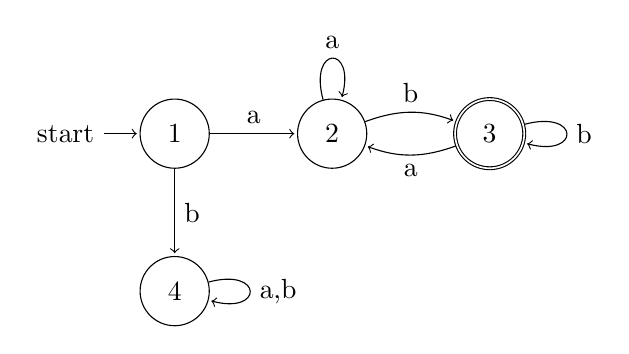
\begin{tikzpicture}[shorten >=1pt,node distance=2cm,on grid,auto] 
	   \node[state,initial] (q_0)   {$1$};
	   \node[state] (q_1) [right=of q_0] {$2$}; 
	   \node[state,accepting] (q_2) [right=of q_1] {$3$};
	   \node[state] (q_3) [below=of q_0] {$4$}; 
	    \path[->] 
	    (q_0) edge node {a} (q_1)
	    	  edge node {b} (q_3)
	    (q_1) edge [bend left=20] node  {b} (q_2)
	          edge [loop above] node {a} ()
	    (q_2) edge [loop right] node {b} ()
	          edge [bend left=20] node {a} (q_1)
	    (q_3) edge [loop right] node {a,b} ();
	\end{tikzpicture} 
	\caption{Figure 5}
\end{center}
\end{figure}


The string entered must begin with an $a$, and must end with a $b$.
When a string begins with $a$, it is impossible to state 4.
When a string does not conclude with $b$, it will finish at state 2.

\section{Transition matrix for automata in figure 6 labeled A,B}

\[ A = \left( \begin{array}{cccc}
0 & 1 & 0 & 0 \\
0 & 1 & 0 & 0 \\
0 & 1 & 0 & 0 \\
0 & 0 & 0 & 1 \end{array} \right)\] 

\[ B = \left( \begin{array}{cccc}
0 & 0 & 0 & 1 \\
0 & 0 & 1 & 0 \\
0 & 0 & 1 & 0 \\
0 & 0 & 0 & 1 \end{array} \right)\] 

\[ AB = \left( \begin{array}{cccc}
0 & 0 & 1 & 0 \\
0 & 0 & 1 & 0 \\
0 & 0 & 1 & 0 \\
0 & 0 & 0 & 1 \end{array} \right)\] 

\[ BA = \left( \begin{array}{cccc}
0 & 0 & 0 & 1 \\
0 & 1 & 0 & 1 \\
0 & 1 & 0 & 1 \\
0 & 0 & 0 & 1 \end{array} \right)\] 

\[ A^2 = \left( \begin{array}{ccccc}
0 & 1 & 0 & 1 \\
0 & 1 & 0 & 0 \\
0 & 1 & 0 & 0 \\
0 & 0 & 0 & 1 \end{array} \right)\] 

\[ B^2 = \left( \begin{array}{ccccc}
0 & 0 & 0 & 1 \\
0 & 0 & 1 & 0 \\
0 & 0 & 1 & 0 \\
0 & 0 & 0 & 1 \end{array} \right)\] 

\subsection{Description of transition matrices for the automata in Figure 6}
These matrices represent beginning and end states for a finite automata. For matrix index ${a_i}_j$, we view row
$i$ as the beginning state, and $j$ as the end state. For example, matrix $A$ represents the act of feeding a 
single $a$ character into the automata. Beginning at row $1$, state $1$ will have the end result of traveling  
to column $2$, state $2$ of the automata. This idea extends to the transition matrix $A^2$, which feeds two $a$ 
characters into the automata. The same applies for $B^2$ and all other cases of transition matrices as well. 
This idea also extends to the case where we multiply transition matrix $A$ by transition matrix $B$. 
This new transition matrix $AB$ represents the event that two characters $a$ and $b$ are put into the 
finite automata. Again, beginning at row $1$, the end result will be that the end state will result at state $3$.


\section{Finite automata that accepts all strings that have even numbers of $a's$ and $b's$}

\begin{center}
	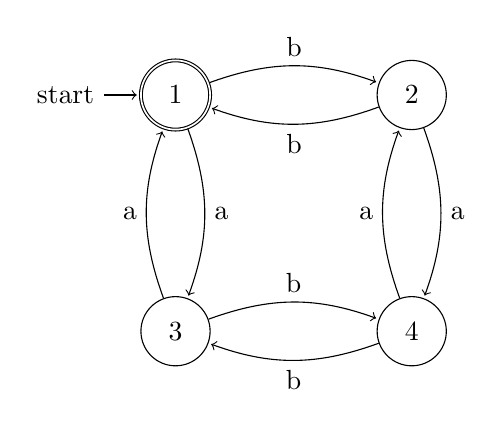
\begin{tikzpicture}[shorten >=1pt,node distance=3cm,on grid,auto] 
	   \node[state,initial, accepting] (q_0)   {$1$};
	   \node[state] (q_1) [right=of q_0] {$2$};
	   \node[state] (q_2) [below=of q_0] {$3$}; 
	   \node[state](q_3) [right=of q_2] {$4$}; 
	    \path[->] 
	    (q_0) edge  [bend left=20] node {b} (q_1)
	    	  edge  [bend left=20] node {a} (q_2)
	    (q_1) edge  [bend left=20] node {b} (q_0)
	          edge  [bend left=20] node {a} (q_3)
	    (q_2) edge  [bend left=20] node {b} (q_3)
	          edge  [bend left=20] node {a} (q_0)
	    (q_3) edge  [bend left=20] node {b} (q_2)
	          edge  [bend left=20] node {a} (q_1);
	\end{tikzpicture} 
\end{center}


\subsection{Transition matrices for previous automata}

\[ A = \left( \begin{array}{cccc}
0 & 0 & 1 & 0 \\
0 & 0 & 0 & 1 \\
1 & 0 & 0 & 0 \\
0 & 1 & 0 & 0 \end{array} \right)\] 

\[ B = \left( \begin{array}{cccc}
0 & 1 & 0 & 0 \\
1 & 0 & 0 & 0 \\
0 & 0 & 0 & 1 \\
0 & 0 & 1 & 0 \end{array} \right)\] 

\[ AB = \left( \begin{array}{cccc}
0 & 0 & 0 & 1 \\
0 & 0 & 1 & 0 \\
0 & 1 & 0 & 0 \\
1 & 0 & 0 & 0 \end{array} \right)\] 

\[ BA = \left( \begin{array}{cccc}
0 & 0 & 0 & 1 \\
0 & 0 & 1 & 0 \\
0 & 1 & 0 & 0 \\
1 & 0 & 0 & 0 \end{array} \right)\] 

\[ A^2 = \left( \begin{array}{ccccc}
1 & 0 & 0 & 0 \\
0 & 1 & 0 & 0 \\
0 & 0 & 1 & 0 \\
0 & 0 & 0 & 1 \end{array} \right)\] 

\[ B^2 = \left( \begin{array}{ccccc}
1 & 0 & 0 & 0 \\
0 & 1 & 0 & 0 \\
0 & 0 & 1 & 0 \\
0 & 0 & 0 & 1 \end{array} \right)\] 

\subsection{Eigenvalues and eigenvectors}

  \begin{center}
  \textbf{$A$}
  \end{center}

  \begin{center}
  \begin{tabular}{ c c c p{5cm} }
    $\lambda_1$ & $\rightarrow$ & -1 \\        
    $\lambda_2$ & $\rightarrow$ & -1 \\
    $\lambda_3$ & $\rightarrow$ &  1 \\
    $\lambda_4$ & $\rightarrow$ &  1 \\
  \end{tabular}
  \end{center}

  \begin{center}
  $\vec{x}_1 = \begin{pmatrix}0\\ -1 \\ 0 \\ 1 \end{pmatrix}$
  $\vec{x}_2 = \begin{pmatrix}-1\\ 0 \\ 1 \\ 0 \end{pmatrix}$
  $\vec{x}_3 = \begin{pmatrix}0\\ 1 \\ 0 \\ 1 \end{pmatrix}$
  $\vec{x}_4 = \begin{pmatrix}1\\ 0 \\ 1 \\ 0 \end{pmatrix}$
  \end{center}

\pagebreak

  \begin{center}
  \line(1,0){250}\\
  \textbf{$B$}
  \end{center}

  \begin{center}
  \begin{tabular}{ c c c p{5cm} }
    $\lambda_1$ & $\rightarrow$ & -1 \\        
    $\lambda_2$ & $\rightarrow$ & -1 \\
    $\lambda_3$ & $\rightarrow$ &  1 \\
    $\lambda_4$ & $\rightarrow$ &  1 \\
  \end{tabular}
  \end{center}

  \begin{center}
  $\vec{x}_1 = \begin{pmatrix}0\\ 0 \\ -1 \\ 1 \end{pmatrix}$
  $\vec{x}_2 = \begin{pmatrix}-1\\ 1 \\ 0 \\ 0 \end{pmatrix}$
  $\vec{x}_3 = \begin{pmatrix}0\\ 0 \\ 1 \\ 1 \end{pmatrix}$
  $\vec{x}_4 = \begin{pmatrix}1\\ 1 \\ 0 \\ 0 \end{pmatrix}$
  \end{center}

  \begin{center}
  \line(1,0){250}\\
  \textbf{$AB = BA$}
  \end{center}

  \begin{center}
  \begin{tabular}{ c c c p{5cm} }
    $\lambda_1$ & $\rightarrow$ & -1 \\        
    $\lambda_2$ & $\rightarrow$ & -1 \\
    $\lambda_3$ & $\rightarrow$ &  1 \\
    $\lambda_4$ & $\rightarrow$ &  1 \\
  \end{tabular}
  \end{center}

  \begin{center}
  $\vec{x}_1 = \begin{pmatrix}-1\\ 0 \\ 0 \\ 1 \end{pmatrix}$
  $\vec{x}_2 = \begin{pmatrix}0\\ -1 \\ 1 \\ 0 \end{pmatrix}$
  $\vec{x}_3 = \begin{pmatrix}1\\ 0 \\ 0 \\ 1 \end{pmatrix}$
  $\vec{x}_4 = \begin{pmatrix}0\\ 1 \\ 1 \\ 0 \end{pmatrix}$
  \end{center}

  \begin{center}
  \line(1,0){250}\\
  \textbf{$A^2 = B^2$}
  \end{center}

  \begin{center}
  \begin{tabular}{ c c c p{5cm} }
    $\lambda_1$ & $\rightarrow$ & 1 \\        
    $\lambda_2$ & $\rightarrow$ & 1 \\
    $\lambda_3$ & $\rightarrow$ & 1 \\
    $\lambda_4$ & $\rightarrow$ & 1 \\
  \end{tabular}
  \end{center}

  \begin{center}
  $\vec{x}_1 = \begin{pmatrix}0\\ 0 \\ 0 \\ 1 \end{pmatrix}$
  $\vec{x}_2 = \begin{pmatrix}0\\ 0 \\ 1 \\ 0 \end{pmatrix}$
  $\vec{x}_3 = \begin{pmatrix}0\\ 1 \\ 0 \\ 0 \end{pmatrix}$
  $\vec{x}_4 = \begin{pmatrix}1\\ 0 \\ 0 \\ 0 \end{pmatrix}$
  \end{center}

\subsection{Importance of eigenvalues and eigenvectors to automata}

The absolute value of the eigenvalues for each calculated matrix is one. The eigenvalues for $A$, $B$, $AB$, and 
$BA$ are symmetric. This represents that there are multiple nodes that have the
same properties of adjacency.

\section{Finite automata that accepts all strings with a substring $aaa$}

\begin{center}
	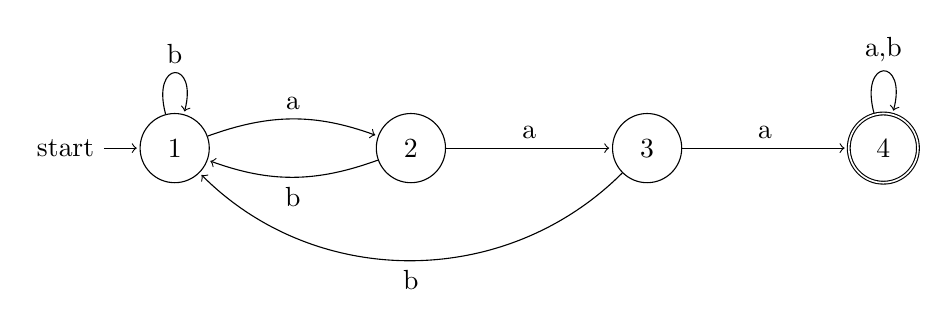
\begin{tikzpicture}[shorten >=1pt,node distance=3cm,on grid,auto] 
	   \node[state,initial] (q_0)   {$1$};
	   \node[state] (q_1) [right=of q_0] {$2$};
	   \node[state] (q_2) [right=of q_1] {$3$}; 
	   \node[state, accepting](q_3) [right=of q_2] {$4$}; 
	    \path[->] 
	    (q_0) edge  [bend left=20] node {a} (q_1)
	          edge  [loop above]    node {b} ()
	    (q_1) edge  [bend left=20] node {b} (q_0)
	          edge  node {a} (q_2)
	    (q_2) edge  node {a} (q_3)
	          edge  [bend left=45] node {b} (q_0)
	    (q_3) edge  [loop above] node {a,b} ();
	\end{tikzpicture} 
\end{center}

\[ A = \left( \begin{array}{cccc}
0 & 1 & 0 & 0 \\
0 & 0 & 1 & 0 \\
0 & 0 & 0 & 1 \\
0 & 0 & 0 & 1 \end{array} \right)\] 

\[ B = \left( \begin{array}{cccc}
1 & 0 & 0 & 0 \\
1 & 0 & 0 & 0 \\
1 & 0 & 0 & 0 \\
0 & 0 & 0 & 1 \end{array} \right)\] 

\[ AB = \left( \begin{array}{cccc}
1 & 0 & 0 & 0 \\
1 & 0 & 0 & 0 \\
0 & 0 & 0 & 1 \\
0 & 0 & 0 & 1 \end{array} \right)\] 

\[ BA = \left( \begin{array}{cccc}
0 & 1 & 0 & 0 \\
0 & 1 & 0 & 0 \\
0 & 1 & 0 & 0 \\
0 & 0 & 0 & 1 \end{array} \right)\] 

\[ A^2 = \left( \begin{array}{ccccc}
0 & 0 & 1 & 0 \\
0 & 0 & 0 & 1 \\
0 & 0 & 0 & 1 \\
0 & 0 & 0 & 1 \end{array} \right)\] 

\[ B^2 = \left( \begin{array}{ccccc}
1 & 0 & 0 & 0 \\
1 & 0 & 0 & 0 \\
1 & 0 & 0 & 0 \\
0 & 0 & 0 & 1 \end{array} \right)\] 

\subsection{Eigenvalues and eigenvectors}

  \begin{center}
  \textbf{$A$}
  \end{center}

  \begin{center}
  \begin{tabular}{ c c c p{5cm} }
    $\lambda_1$ & $\rightarrow$ & 1 \\        
    $\lambda_2$ & $\rightarrow$ & 0 \\
    $\lambda_3$ & $\rightarrow$ & 0 \\
    $\lambda_4$ & $\rightarrow$ & 0 \\
  \end{tabular}
  \end{center}

  \begin{center}
  $\vec{x}_1 = \begin{pmatrix}1\\ 1 \\ 1 \\ 1 \end{pmatrix}$
  $\vec{x}_2 = \begin{pmatrix}1\\ 0 \\ 0 \\ 0 \end{pmatrix}$
  $\vec{x}_3 = \begin{pmatrix}0\\ 0 \\ 0 \\ 0 \end{pmatrix}$
  $\vec{x}_4 = \begin{pmatrix}0\\ 0 \\ 0 \\ 0 \end{pmatrix}$
  \end{center}

  \begin{center}
  \line(1,0){250}\\
  \textbf{$B$}
  \end{center}

  \begin{center}
  \begin{tabular}{ c c c p{5cm} }
    $\lambda_1$ & $\rightarrow$ & 1 \\        
    $\lambda_2$ & $\rightarrow$ & 1 \\
    $\lambda_3$ & $\rightarrow$ & 0 \\
    $\lambda_4$ & $\rightarrow$ & 0 \\
  \end{tabular}
  \end{center}

  \begin{center}
  $\vec{x}_1 = \begin{pmatrix}0\\ 0 \\ 0 \\ 1 \end{pmatrix}$
  $\vec{x}_2 = \begin{pmatrix}1\\ 1 \\ 1 \\ 0 \end{pmatrix}$
  $\vec{x}_3 = \begin{pmatrix}0\\ 0 \\ 1 \\ 0 \end{pmatrix}$
  $\vec{x}_4 = \begin{pmatrix}0\\ 1 \\ 0 \\ 0 \end{pmatrix}$
  \end{center}

  \begin{center}
  \line(1,0){250}\\
  \textbf{$AB$}
  \end{center}

  \begin{center}
  \begin{tabular}{ c c c p{5cm} }
    $\lambda_1$ & $\rightarrow$ & 1 \\        
    $\lambda_2$ & $\rightarrow$ & 1 \\
    $\lambda_3$ & $\rightarrow$ & 0 \\
    $\lambda_4$ & $\rightarrow$ & 0 \\
  \end{tabular}
  \end{center}

  \begin{center}
  $\vec{x}_1 = \begin{pmatrix}0\\ 0 \\ 1 \\ 1 \end{pmatrix}$
  $\vec{x}_2 = \begin{pmatrix}1\\ 1 \\ 0 \\ 0 \end{pmatrix}$
  $\vec{x}_3 = \begin{pmatrix}0\\ 0 \\ 1 \\ 0 \end{pmatrix}$
  $\vec{x}_4 = \begin{pmatrix}0\\ 1 \\ 0 \\ 0 \end{pmatrix}$
  \end{center}

  \begin{center}
  \line(1,0){250}\\
  \textbf{$BA$}
  \end{center}

  \begin{center}
  \begin{tabular}{ c c c p{5cm} }
    $\lambda_1$ & $\rightarrow$ & 1 \\        
    $\lambda_2$ & $\rightarrow$ & 1 \\
    $\lambda_3$ & $\rightarrow$ & 0 \\
    $\lambda_4$ & $\rightarrow$ & 0 \\
  \end{tabular}
  \end{center}

  \begin{center}
  $\vec{x}_1 = \begin{pmatrix}0\\ 0 \\ 0 \\ 1 \end{pmatrix}$
  $\vec{x}_2 = \begin{pmatrix}1\\ 1 \\ 1 \\ 0 \end{pmatrix}$
  $\vec{x}_3 = \begin{pmatrix}0\\ 0 \\ 1 \\ 0 \end{pmatrix}$
  $\vec{x}_4 = \begin{pmatrix}1\\ 0 \\ 0 \\ 0 \end{pmatrix}$
  \end{center}

  \begin{center}
  \line(1,0){250}\\
  \textbf{$A^2$}
  \end{center}

  \begin{center}
  \begin{tabular}{ c c c p{5cm} }
    $\lambda_1$ & $\rightarrow$ & 1 \\        
    $\lambda_2$ & $\rightarrow$ & 0 \\
    $\lambda_3$ & $\rightarrow$ & 0 \\
    $\lambda_4$ & $\rightarrow$ & 0 \\
  \end{tabular}
  \end{center}

  \begin{center}
  $\vec{x}_1 = \begin{pmatrix}-1\\ -1 \\ -1 \\ -1 \end{pmatrix}$
  $\vec{x}_2 = \begin{pmatrix}0\\ 1 \\ 0 \\ 0 \end{pmatrix}$
  $\vec{x}_3 = \begin{pmatrix}1\\ 0 \\ 0 \\ 0 \end{pmatrix}$
  $\vec{x}_4 = \begin{pmatrix}0\\ 0 \\ 0 \\ 0 \end{pmatrix}$
  \end{center}

  \begin{center}
  \line(1,0){250}\\
  \textbf{$B^2$}
  \end{center}

  \begin{center}
  \begin{tabular}{ c c c p{5cm} }
    $\lambda_1$ & $\rightarrow$ & 1 \\        
    $\lambda_2$ & $\rightarrow$ & 1 \\
    $\lambda_3$ & $\rightarrow$ & 0 \\
    $\lambda_4$ & $\rightarrow$ & 0 \\
  \end{tabular}
  \end{center}

  \begin{center}
  $\vec{x}_1 = \begin{pmatrix}0\\ 0 \\ 0 \\ 1 \end{pmatrix}$
  $\vec{x}_2 = \begin{pmatrix}1\\ 1 \\ 1 \\ 0 \end{pmatrix}$
  $\vec{x}_3 = \begin{pmatrix}0\\ 0 \\ 1 \\ 0 \end{pmatrix}$
  $\vec{x}_4 = \begin{pmatrix}0\\ 1 \\ 0 \\ 0 \end{pmatrix}$
  \end{center}

\subsection{Importance of eigenvalues and eigenvectors to automata}

\end{document} 